\chapter[Vulnerability assessment]{Vulnerability assessment: a starter's guide}
\label{ch:vuln_assessment}

In order to search for vulnerabilities, we need a vast number of tools, and to even scratch the surface of one of them we would need hundreds of hours. This chapter is only meant as a fast introduction, as we have neither the time nor the possibility to see all of them or to go into details for any of them.
 
Generally speaking, there is not a single tool or solution, so before doing a vulnerability assessment we need to make a plan so as to know more or less what kind of problems we should look after. Usually, some \textbf{Linux distributions} specifically made for vulnerability assessment are normally employed for this operation, and they are often mistaken for attacking tools (they can be used for that, too, but have been created for white hat purposes). Mind that while attackers have to careful to avoid being tracked, in a vulnerability assessment the tester does not care if he or she is identified. In practical terms, this means that using standard vulnerability assessment tools for hacking live systems (with malicious intents) is a very bad idea, because they do not provide protection out of the box.

A quick Google search will reveal the existence of many Linux-based tools, like Kali Linux, Parrot, Samurai, Pentoo, DEFT and BlackArch; like mentioned above, even though they are not equivalent to each other, there is not one that is better than the others, either. They could be better only with respect to certain vulnerability assessment aspects. We should try many of them in order to find which one we like or need the most.

Remember that when performing a penetration test we should always document everything that we are doing, as we do not want random stuff to happen (although if we cannot remember what we have done, then maybe we are not very good at what we are doing). This can be done by either using pen and paper, or by taking screenshots and using an advanced notepad.

Last but not least, keep in mind that penetration test tools \textbf{require time}. Like, time for booting up, searching for devices, and so on.
 
%----------------------------------------------------------------------------------------

\section{Kali Linux}
\textbf{Kali Linux} is probably the best-known vulnerability assessment tool, and is marketed as an advanced penetration testing open source distro\footnote{Penetration testing is equivalent to vulnerability assessment, because if we are able to break a system, then it has some vulnerability.}.

Although on paper it is easy to install, in practice this is a rather complex (or at least time-consuming) process. There are many ways of installing it, on different devices:

\begin{itemize}
	\item as an \textbf{operating system} on a dedicated machine or in a virtual environment (e.g. VirtualBox, VMware, etc.);
	\item on the Windows Subsystem for Linux (\textbf{Win-KeX} version), which allows its virtualization on a Windows 10 machine without the overhead of a traditional virtual machine;
	\item on specific Android devices (\textbf{Kali NetHunter});
	\item on an \textbf{ARM device}, like Raspberry Pi, Banana Pi, Pine64 or Chromebooks (good for injecting data in a network, but not indicated for cracking passwords\footnote{Attempting to crack a password with one of these devices would be “slower than prof. Pecorella in the morning without a coffee”.}).
\end{itemize}
 
%-------------------------------------------

\subsection{Kali Linux installation}
The following is a brief collection of tips \& tricks learned by prof. Pecorella the night before this lesson while installing Kali Linux from scratch on VirtualBox\footnote{While installing Kali from scratch (the distribution image), it is better to set the network on “not attached”, otherwise the installation could hang. A guide can be found at \url{https://www.ojoiszy.com/install-kali-linux-on-virtualbox}.}. Note that there exist pre-made Kali Linux VirtualBox (or VMware) images\footnote{\url{ https://www.offensive-security.com/kali-linux-vm-vmware-virtualbox-image-download}} (which are actually recommended for the sake of simplicity).

First of all, before installing Kali Linux we should make sure that our system has enough CPU cores and, most importantly, \textbf{good network interface devices}.

%----------------------

\subsubsection*{Network adapters}
VirtualBox can give to each machine up to four different NICs; by default it uses a \textbf{NAT}, meaning that the virtualized machine will be NATted by our own computer (the host), and thus will access a network internal to VirtualBox itself. This configuration leaves much to desire for, as it severely limits penetration testing, since other devices in the host’s network will \textit{not} be seen as link local.

The \textbf{bridge adapter} option splits the NIC between the test machine and the host, and the guest machine will be in the real network. However, this will put extra stress on the network card because it will (probably) get two different MAC addresses and (surely) two different IP addresses - if it is IPv4, otherwise in IPv6 it will get a \textit{zillion} more. What is worse, Kali Linux will see everything in the network, and if we make some mistake we could poke the wrong device or the Internet itself - which could not only pose a real danger for our own security, but would also cause the firewall or other similar applications to start complaining, since they will see us as an attacker. So, to put it shortly: bridge adapter mode should only be used if we really know what we are doing, or if we really want a slap from the network admin.
 
Another (highly suggested) option is called \textbf{internal network}: it creates a virtualized switched network inside VirtualBox, which is exactly what we need in order to experiment with different virtual machines without causing any damage to live devices.

A good configuration can be achieved by using two NICs: a bridged adapter and an internal network. This allows to attack machines on the internal network while also being able to access the Internet (just be careful to not give the wrong command in the wrong network).

%----------------------

\subsubsection*{Metapackages}
During install, Kali Linux also asks the user what kind of installation he/she wants, if either the full version or a reduced one. This choice is not very important, as what it really does is just specifying which metapackages will be installed.

A \textbf{metapackage} is a package containing other packages, much like a list of things that must be installed. Remember that in Linux, a \textbf{package} is a sort of program that installs stuff in the right place, just like a Windows installer.

\vspace{0.5em}

\emph{Example} \texttt{kali-linux-forensic} provides the most used tools for forensics analysis, the process of analyzing a device (probably given to us by the authorities) without modifying or compromising it in any way.

\texttt{kali-linux-gpu} offers tools optimized for GPU execution.

\texttt{kali-linux-rfid} contains tools to check on or attack RFID devices.

\vspace{0.5em}
 
Kali Linux is built around metapackages, so basically during the install process we choose what tools we are going to find in the final install, but we are free to uninstall, modify or add new metapackages at any time. The only relevant consideration is the one regarding the amount of space occupied by these packages, as certain devices (e.g. ARM) might not have enough space for a full install, which is typically 80+ GB ($\sim$ 30 GB when reduced). We should have around 128 GB of free space, and keep in mind that we will also need space for collected data.

\vspace{0.5em}

\emph{Example} Prof. Pecorella used for his lesson the \texttt{kali-linux-large} metapackage, which uses 13 GB - not dramatically high.

%----------------------

\subsubsection*{Desktop environment}
During installation, Kali Linux asks which kind of graphic setup we want; the default option is the \textbf{Xfce desktop environment}, although one could use GNOME or other environments. The point here is that we do not need this OS to look pretty, but to be fast, and the best choice for achieving this is Xfce, as it is the least demanding in terms of resources. As a bonus, it also comes with a menu which already groups applications in categories (figure \ref{fig:xfce}), making it easier for new users to find what they need\footnote{Some tools are repeated in different groups because they can be used for different things. Note that what we find in this menu depends on the installed metapackages.}.

\begin{figure}[h]
    \centering
    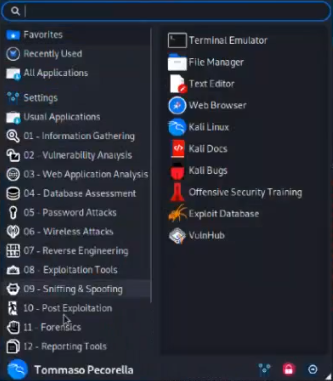
\includegraphics[scale=1]{img/xfce.png}
    \decoRule
    \caption{Xfce desktop environment main menu.}
    \label{fig:xfce}
\end{figure}

%-------------------------------------------

\subsection{Installation vs. virtualization}
The restriction on the number of devices supporting Kali NetHunter originates from the fact that in order to do penetration testing we need to access the transmission devices (Wi-Fi, Bluetooth and Ethernet) at their lowest level; the NICs must be capable of enabling promiscuous mode and not lose packets, which in turn means having good drivers - something not as obvious as one might think. In fact, many NIC manufacturers sell specific penetration testing devices (like Wi-Fi cards).

Moreover, while all this is possible with normally installed operating systems, penetration testing becomes more difficult if not impossible on virtualized distros, which run on a layer of software that hides the real workings of the physical NIC. As a consequence, running any Kali Linux distro in a virtual environment like VirtualBox will most probably not be as effective as running it natively on a computer.

%-------------------------------------------

\subsection{Metasploit}
\textbf{Metasploit} is what made Kali Linux famous. It is not a simple tool, as it has tons of functionalities, and mastering it requires a lot of time, knowledge and patience. As misconceptions go, Metasploit is \textit{not} Kali Linux: they are completely different projects, and it is much like mistaking Ubuntu for OpenOffice.

Metasploit is nothing more than a huge Ruby\footnote{Ruby is a programming language particularly interesting for its expressiveness, strength in payload and string generation and the ability to easily install plugins, which make it well suited for writing exploit-related applications and scripts.} program installed on Kali Linux. It also works on Ubuntu, macOS and Windows, but since it uses a number of other tools, installing it from scratch on a different OS would not only be difficult, but would also make us lose the point of running it on an OS specifically optimized for penetration testing. 

Metasploit per se looks horrible, as it only offers a command line interface (yay). In order to learn how to use this tool (if we are serious about it) we should find a book about Metasploit only. A good choice is \textbf{\textit{Metasploit Unleashed}}\footnote{Freely available at \url{https://www.offensive-security.com/metasploit-unleashed/}.} by Offensive Security (Metasploit’s and Kali Linux’ creators), which starts with the basic commands and highly recommended stuff before diving into more complex topics.
 
Just by looking at this book’s index, we can deduce that Metasploit can be used to develop exploits (i.e. ways to leverage a vulnerability), trojans, backdoors, and tons of similar applications. Currently Metasploit has 2070 exploits, 1123 auxiliary tools and other stuff: although not user-friendly, it is incredibly powerful.

%----------------------

\subsubsection{Armitage}
\textbf{Armitage} is the best-known GUI for Metasploit. It looks neat and it is a nice tool, but we should be wary of it because like all GUIs it only offers a subset of the options of a CLI. For this reason, we should first find vulnerabilities using the command line interface, and only after doing this we could use Armitage for exploiting our findings, otherwise we might unknowingly leave out vulnerabilities because the GUI did not have the option to look for them.

\vspace{0.5em}

\emph{Example} Using Armitage instead of Metasploit is like using the Linux GUI for renaming files: while it is neat and fast for renaming one or two files, it would require a lot of time to use on hundreds of files at a time. Vice versa, the same operation can be done with a single command through the terminal. We do need to know very well the command line scripting language, but it is a completely different world.

\vspace{0.5em}

%-------------------------------------------

\subsection{Kali NetHunter}
\textbf{Kali NetHunter} is a free and open source mobile penetration testing platform for Android devices. It is a specialized version of Kali Linux that installs on a smartphone the tools for \textbf{nethunting}, the process of searching for wireless networks like Bluetooth or Wi-Fi.

The NetHunter distro is used for gathering information about, for example, which devices are on, which Wi-Fi networks are active and where is located an access point (this one by measuring the RSSI\footnote{The received signal strength indicator (RSSI) is a measurement of the power present in a received radio signal.}). This data, collected while going around, can be later used for a physical attack.

While being quite interesting for its \textbf{portability}, Kali NetHunter’s drawback is that it can only be installed on a handful of \textbf{very specific devices} - to the point that some of them are very valuable in the world of penetration testing, in spite of being rather old.

%----------------------------------------------------------------------------------------

\section{Metasploitable 2}
Besides the Kali Linux distro we need another machine on the same virtual network on which to conduct our experiments. There are mainly three options for doing this:

\begin{itemize}
	\item create a \textbf{Ubuntu} or \textbf{Windows} virtual machine (or any other similar operating system). The problem with this kind of configuration is that if the system is up to date, chances are that we will not find any usable vulnerability;
	\item use \textbf{Metasploitable 2}, a Linux distro containing a number of vulnerabilities, specifically created for practicing penetration testing; it can be set up in a very short time, and has an extensive on-line guide\footnote{Freely available at \url{https://docs.rapid7.com/metasploit/metasploitable-2-exploitability-guide}.};
	\item trying to use \textbf{Metasploitable 3}, although it is much more difficult to install than Metasploitable 2 as it uses Windows Server 2008 (kind of old, but still interesting). Note that for the virtualization part Metasploitable 3 uses Vagrant\footnote{Vagrant is a product for building and maintaining virtual machines that can be later used in virtualized environments, like VirtualBox or VMware.}, which has quite unrealistic timeouts on the download of packages and components, and might cause applications to fail if the system does not have a very fast HDD or Internet connection. 
\end{itemize}

Kali Linux, being made for penetration testing (research purposes) and \textit{not} attacking, does not come out of the box with tools that allow to exploit unpatched (known) vulnerabilities on live systems.

Exploitation tools for known and patched vulnerabilities are only included to test if the patch has been correctly applied. Mind that a penetration test suite can be programmed and extended at will to exploit new vulnerabilities, but we will have to put some effort in it and we will have to know what we are doing, meaning that it is not stuff for script kiddies who could damage things without realizing it.

For this reason, as well as for its simplicity, the best machine on which to perform experiments is Metasploitable 2.

%-------------------------------------------

\subsection{Exploits in practice} 
What is the effect of an exploit in practice? Let us try one from the Metasploitable 2 guide. In a Kali Linux terminal, we can send the following command (where the example IP address must be replaced with the one belonging to the Metasploitable 2 machine):

\begin{align*}
\centering
\texttt{rlogin -l root 192.168.45.217}
\end{align*}
 
We just logged in a remote machine without it showing any prompt to the user, because the remote login feature is configured incorrectly.

Generally speaking, we should always poke even the simplest exploits, because we never know when we might have forgotten something in the machine’s configuration.

\vspace{0.5em}

\emph{Example} SQL databases are phenomenally vulnerable, so much that one will never understand how vulnerable they are unless someone attacks them. For this reason, these databases should be installed on a very well protected network, because they are full of backdoors.

\vspace{0.5em}

%----------------------------------------------------------------------------------------

\section{Viruses}
The term \textbf{\textit{virus}} by itself is irrelevant; what really interests us is the broader category of viruses but also \textbf{worms}, \textbf{trojans} and other \textbf{malware} or, in other words, any automated attack vector that can \textbf{replicate itself} and \textbf{spread} without explicit user consent.

These programs are pieces of software able to install themselves in a target machine without any interaction from the user, by leveraging network and/or hardware vulnerabilities and features (e.g. USB pens or cellphones). After installation, viruses normally proceed with infecting other machines as soon as they come in contact with another exploitable system.

Thirty years ago, viruses were extremely common; in fact, they were so frequently encountered that some universities had courses teaching how to develop them, since they require knowledge of advanced programming techniques. That was because in order to write a virus or a worm one must know exactly how the target machine works, and be able to write small, efficient code capable of hiding and obfuscating itself from the operating system in the most creative manners. Of course, after a while professors realized that however interesting, these courses were better not be regularly taught for security reasons.

\vspace{0.5em}

\emph{Joke} Is Windows 95 a virus? Clearly not, because a virus has well written code, occupies little disk space and is efficient.

\vspace{0.5em}

Nowadays viruses and worms have almost transitioned to a sort of on-demand thing: there is plenty of tools on the Internet allowing a person to create one (e.g. Kali Linux contains some \textbf{weaponization} tools).

Defense against viruses is only slightly different from defense against human attackers, with the advantage (over a human being) that viruses are \textbf{highly predictable}: once we know how they operate, finding them is rather simple. In order to do this we can use the usual network security solutions, along with \textbf{personal intrusion detection systems}. These are needed because viruses spread and obfuscate themselves in seemingly innocent files, like e-mail attachments, Microsoft Word macros, etc., \textbf{bypassing the network security measures} by exploiting an active error on the user’s part. An \textbf{antivirus} is able to detect them by blacklisting certain filetypes and actively scanning for them in the payload of the most common applications.

Generally, the best defense against viruses is to \textbf{not open suspicious files} or click on doubtful ads, like those claiming that the user has won a ten million dollars prize or received an inheritance from an uncle he/she did not know about.

%----------------------------------------------------------------------------------------

\section{Antiviruses, or intrusion detection systems}
So far, we have not talked about \textbf{antiviruses}, or how we fit a complete security solution in a security area.

Suppose that we have defined a security area, which by definition is a portion of the network that is isolated from the rest of the network; this area has a certain kind of traffic with a certain kind of users that are allowed to do some stuff, and it also has to block traffic that is not supposed to pass from one side to another. But what about the traffic \textit{inside} the security area?

We need something that is able to monitor internal traffic and raise an alarm. \textbf{Intrusion detection systems} (\textbf{IDSs}) are computer programs (either machines or software) that inspect the flow of data between computers and look for suspicious activity\footnote{Remember, orange is sus.}. But how is “suspicious activity" defined, and what do we do afterwards?
 
The answer is not very obvious. There is a conceptual difference between the two big types of IDSs: rule-based and behavioral-based. They both have their pros and cons;  pattern matching systems are perfect for finding unknown attacks (those that do not have a defined pattern yet), although variations of an attack can easily fool the rules. Behavior-based IDSs are not much more flexible, as they might go crazy with people with ever-changing, unpredictable behavior.

Another problem is that of \textit{where} to perform the traffic analysis:

\begin{itemize}
    \item \textbf{spilling data from the switch} is an option, but in order to do this we need special, high-performance and high-speed switch ports, as well as a computer capable of analyzing large amounts of packets (e.g. 40 Gb/s) without losing them. Usually, normal computers cannot even grab 1 Gb/s of packets, even if the port receives it, because they have to be transferred to the bus, then the CPU and HDD, and it is critical for an IDS that no packets are lost, otherwise patterns cannot be found;
    \item \textbf{offloading tasks elsewhere} is the distributed alternative, as it allows to lighten the task of the piece of software that is performing the screening.
\end{itemize}

%-------------------------------------------

\subsection{Rule-based IDSs}
Rule-based IDSs inspect the traffic, try to find patterns in it and eventually raises an alarm. A \textbf{pattern} is a command or sequence of commands that are not supposed to be received under normal conditions; some examples are:

\begin{itemize}
	\item a packet’s content (even scattered among many packets);
	\item a sequence of packets (like those in a SYN flood or port scanning);
\end{itemize}

Rule-based IDSs, like all systems with rules, will always find many false positives (something that matches a rule but is harmless) and false negatives (something that should have been marked as suspicious, but has not). Ideally in IDSs we want to minimize the number of false negatives at the expense of having more false positives.

%-------------------------------------------

\subsection{Behavioral-based IDSs} 
Behavioral-based IDSs analyze the regular incoming and outgoing traffic and raise an alarm whenever they find something different from the usual stuff. Now, what does “regular” mean? It means whatever the user does during his or her everyday use of the network and computer. This behavior is not a property of the security area, but of the user; we can teach an IDS what it consists of by means of neural networks.

%-------------------------------------------

\subsection{Famous IDSs}
There are three main IDSs: Snort, Suricata and Zeek.

%----------------------

\subsubsection*{Snort}
Also called \textit{the pork}\footnote{At least by prof. Pecorella, but I found it funny enough to put it here.}, Snort sniffs packets.

It is an open source project (somewhat going commercial though), and is becoming the \textit{de facto} standard for rule-based IDSs. It is kinda simple to install; the actual problem lies in its configuration (much like what happens with firewalls), because there are a zillion rules, each of them relevant for specific OSs and setups. In order to properly use Snort we must check all the rules that apply to our environment and disable the others (since the more rules it has, the slower it becomes): if we get tens of warnings about attacks regarding Windows 95, and we are not running this OS, we have probably made some mistake in the configuration.

Since rules are so important, and writing a Snort rule is extremely hard, we really want to rely on the work done by somebody else - and this is where it becomes commercial, as the open source version allows the download of rules of the past month instead of the updated ones.

%----------------------

\subsubsection*{Suricata}
Suricata is Snort’s competitor, and it can even use the same sets of rules. It was born as a multi-threaded alternative to Snort, but since the latter has become multi-threaded, too, the use of one instead of the other is only relevant up to a certain point.

Suricata is also marketed as an \textbf{intrusion prevention system}, but mind that it does not prevent anything: at best, it could prevent an attack from spreading, but not from happening.
 
A detection system sends the user us an e-mail or SMS; it is developed to be hidden in the network, so as to avoid that attackers hide from it. A prevention system does the same, but instead of sending an alarm to a human that will have to take a countermeasure, it does it automatically: for example if it sees a suspicious ARP flooding or poisoning attack from one port of the switch, it disables that port. In order to make it work correctly it must be paired through a communication channel with the switches and the firewalls in a configuration management system; note that false positives are a lot worse in this case, as the IDS can block the traffic without the user’s intervention.

%----------------------

\subsubsection*{Zeek}
The third, even more complete and specialized solution, is Zeek, formerly known as Bro. Zeek was created because Snort and Suricata used to gather all the traffic in one point and process it there, making it a very sensitive point. Zeek places instead \textbf{sensors} in multiple parts of the network, have them do some screening and then send the already digested stuff to another system. Basically, it was born to be distributed and used in huge networks like fiber optic gigabit Ethernet cables, where normal IDSs were not even able to begin analyzing traffic.

Zeek is rule-based, too, but unlike Suricata it does not support Snort rules.
 
%-------------------------------------------

\subsection{Final considerations about IDSs}
At the end of the day, what is the role of personal intrusion detection systems, like antiviruses?
Are they effective, and are they a real part of a comprehensive network security solution? The answer is: yes, they are. However, in order to be considered part of this solution, they must be part of an ecosystem. If we find a virus on a computer, the role of the antivirus is not just to take it down, but also to alert all the other computers and systems that it found something suspicious.

A comprehensive solution should also look at the processes that have run in the past by checking the system logs. \textbf{System log analysis} is a very powerful technique that allows to spot problems in a computer configuration (what processes have been executed, holes because somebody erased the logs, etc.). For this reason firewalls should employ logging, as they might block an attack, but they cannot know if there was something else going on. We must, however, pay attention to logs, because they might generate too much data. Needless to say, nowadays the most advanced technology uses AI for log and traffic analysis, but it still is an open problem, and for privacy reasons, too (the more data we collect, the less privacy the users get). This is what basically differentiates a firewall from an IDS: while firewall only analyze packets, IDSs also take a look at the logs.

%----------------------------------------------------------------------------------------

\section{Internet of Things security}
\textbf{Security in Internet of Things systems is a touchy problem}.

Some years ago, it was thought that IoT devices represented a problem in the sense that they were too small and not powerful enough to efficiently run security solutions. Nowadays we know that they have CPUs perfectly able to run, for example, a firewall. Nonetheless, the issue with these systems is that traditional network security tools would make them \textbf{run out of battery} in no time.

IoT devices also are usually small and \textbf{lack input}: normally they do not have a wide screen or a keyboard, and more often than not will be left in unattended places, so they are subject to being physically stolen. They commonly use wireless channels, so are subject to packet sniffing, too; and when using multi-hop networks\footnote{ Multi-hop networks are those made by devices which do not directly communicate with a controller within a star network topology, but instead rely on nearby similar devices to transmit their data at low power rates. The technique is used to extend a network’s range in an inexpensive and more efficient manner.}, they open a whole new class of problems.

It is clear then that the main problem of IoT devices is represented by the fact that they cannot - not physically, at least - use the normal security applications that we might think of.

\vspace{0.5em}

\emph{Example} Suppose that we want to secure our phone, and make sure that it has an identity. In order to do this, we can simply install a certificate on it, which we have specifically issued for this phone in particular. Later, when joining a network, we can ask for the certificate and easily identify the phone.

\vspace{0.5em}

Even though the same could be done for IoT devices, usually there are way too many of them to actually make this process feasible. For example, in a single IoT-powered home there could be as many as a hundred devices. We cannot install a certificate on each device: they might not even all have an USB port, or a SSD card, and thus we might have to flash them directly - a cumbersome operation for such a large number of systems.

Instead of using certificates, most companies use \textbf{preinstalled shared certificates}. This means that when a device is \textbf{stolen} or \textbf{decommissioned} (broken and thrashed, which does \textit{not} mean completely erased and irrecuperable), an attacker can \textbf{reverse-engineer} it and \textbf{steal the secret}, so another big problem in IoT devices is represented by the decommissioning process. For efficiency reasons, manufacturers also often take shortcuts in implementing standards and protocols, and sometimes forget to add the core part for security.

\vspace{0.5em}

\emph{Example} Airports have embedded IoT devices on their runways to check for ice; the expected lifetime of those devices is about 20 years – so they are bound to stay there for quite a long time. The same airports, however, are not very strict on decommissioning the devices: anyone could grab and disassemble them, access their memory, find the security data, and then access the network of the airport. The problem is aggravated by the fact that there is no way to change the older devices’ security keys. Moral of the story: always check the companies’ trash because they might contain interesting stuff.

\vspace{0.5em}

\emph{Example} By contrast, the policy for decommissioning security-oriented computers or devices is to open them, take the hard drives apart and physically destroy them (burn them).

\vspace{0.5em}

Last but not least, IoT devices are often sold to the user as plug \& play systems. This feature represents a problem because in order to create a secure and private system we need a network admin, but when this admin is the user itself, more often than not they will not be aware of the security implications of such devices - not because they are stupid, but because they are \textbf{unprepared}. And what is worse is that users do not want to be bored with technical stuff, they just want things to work (meaning that security is pretty much gone).

\vspace{0.5em}

\emph{Example} \textbf{\textit{Alexa, who am I speaking to?}}\footnote{\url{ https://arxiv.org/pdf/1910.14112.pdf}}
This research paper explains that almost half of the surveyed Alexa users (a voice assistant) does not really understand where their data is sent by the device, nor how it is processed and if it could represent a violation of their privacy.

\vspace{0.5em}

From the point of view of network security on the physical and MAC levels there is some hope: the 5G and 6G standards implement very strict and efficient per-user, per-device authentication and authorization systems (for purely greedy reasons, as network operators have the need and desire to strongly identify their users for billing).

At high level (i.e. IP level), however, we will not be able to trust the network, for the same reasons  seen above. Just like telecommunications companies often provide their users with routers containing deactivated firewalls (by default) and do not explain how to properly configure them, IoT devices will most likely keep leaving wide open backdoors in the local network for anyone to exploit\footnote{As the saying goes, \textit{“faucets leak in the plumber’s house”}}.

The \textbf{IoT security issue} will be largely discussed in the coming years, as IoT devices are becoming ever more present in everyday life. For all these reasons IoT systems should be used with great caution (unless we are a network security department that can properly handle them), because they might violate our privacy.

%----------------------------------------------------------------------------------------

\section{Staying updated}
Last but not least, \textbf{always check the news}. We should find a good source of information, like \textit{ArsTechnica}\footnote{\url{https://arstechnica.com/}. It contains a lot of security stuff along with less technical/serious stuff.}. Being updated is vital; if we think that network security has been settled with what we know, we will be eaten alive by the attackers.

%----------------------------------------------------------------------------------------
\section{About free software}
We will probably notice that there is not much information or many (good) how-tos on Metasploit or other tools.

The ecosystem of open source tools evolved over the years in a very complex economic model; to put it simply, open source software developers provide their applications for free, but not their documentation, since they still have to feed their employees and pay the bills. Instead, they offer paid courses, conferences or books to those interested in learning how to properly use their software: basically, “open source” does \textit{not} equal “free”. It is not a scam, but the right way to give back some well-earned money to the people who made certain tools.

There is an important lesson here. We must learn to \textbf{recognize and give kudos} - in terms of money, too – to the people who write open source code. On the other side, we must also learn that \textbf{our time, knowledge and skills are valuable}, and we should always find a way to get something in return for them. Giving stuff away for free might seem nice (and it is), but we have to have a plan to be able to eat and pay the bills at the end of the day.

\begin{figure}[h]
    \centering
    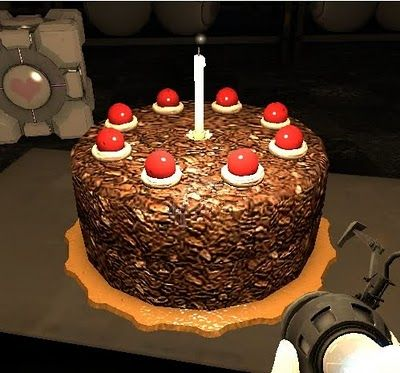
\includegraphics[scale=0.8]{img/portal_cake_meme.jpg}
    \decoRule
    \caption{Dulcis in fundo, the cake. Except it's a lie, just like prof. Pecorella’s \textit{five minutes} breaks (but we love them nonetheless).}
    \label{fig:portal_cake_break}
\end{figure}